\PassOptionsToPackage{table}{xcolor}
\documentclass[12pt,letterpaper,twocolumn,openany,nodeprecatedcode,bg=none]{dndbook}
\usepackage[english]{babel}
\usepackage[utf8]{inputenc}
\usepackage{longtable,booktabs,array}
\usepackage{calc}
\usepackage{etoolbox}
\usepackage{caption}
\usepackage{float}
\usepackage{graphicx}
\usepackage{needspace}
\usepackage{tikz}

% Reset zebra striping at the start of every table
\AtBeginEnvironment{longtable}{\rowcolors{1}{white}{gray!10}\small}
\AtBeginEnvironment{table}{\rowcolors{1}{white}{gray!10}}

\providecommand{\pandocbounded}[1]{#1}
\providecommand{\tightlist}{%
  \setlength{\itemsep}{0pt}\setlength{\parskip}{0pt}}

\captionsetup{labelformat=empty}
\setcounter{secnumdepth}{0}
\setlength{\parindent}{0pt}
\setlength{\parskip}{0.5\baselineskip}
\setlength{\headheight}{15pt}

% Prevent orphaned subsections
\let\oldsubsection\subsection
\renewcommand{\subsection}[1]{%
  \needspace{5\baselineskip}%
  \oldsubsection{#1}%
}

\begin{document}
\onecolumn

      \title{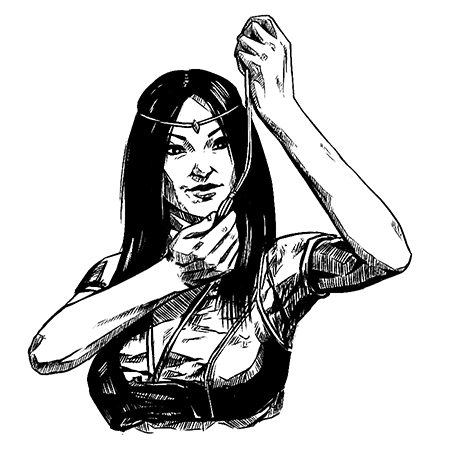
\includegraphics[width=0.9\textwidth,height=0.55\textheight,keepaspectratio]{witchy.jpg}\\[1.5cm]Witch}
  \author{Class Handbook}
\date{}
\maketitle

\clearpage
\thispagestyle{empty}
\null\vfill
\begin{center}{\Large\itshape Your trusty class handbook for fantasy
gaming.}\end{center}
\vfill

\clearpage
\thispagestyle{empty}
\begin{center}
\vspace*{\fill}

\includegraphics[width=\textwidth,height=0.85\textheight,keepaspectratio]{evilWizard.png}\par
\vspace{0.4cm}
{\itshape The right curse can go a long way.}\par
\vspace*{\fill}
\end{center}

\clearpage
\twocolumn

\section{Witch}\label{witch}

\subsection{Core Witch Traits}\label{core-witch-traits}

\needspace{11\baselineskip}

{\def\LTcaptype{none} % do not increment counter
\begin{table}[!htbp]
\centering
\begin{tabular}{@{}
  >{\raggedright\arraybackslash}p{(\linewidth - 2\tabcolsep) * \real{0.4127}}
  >{\raggedright\arraybackslash}p{(\linewidth - 2\tabcolsep) * \real{0.5873}}@{}}
\toprule\noalign{}
\begin{minipage}[b]{\linewidth}\raggedright
\textbf{Primary Ability}
\end{minipage} & \begin{minipage}[b]{\linewidth}\raggedright
Intelligence
\end{minipage} \\
\midrule\noalign{}
\textbf{Hit Points} & 1d4 \\
\textbf{Saving Throw Proficiencies} & Intelligence, Wisdom \\
\textbf{Skill Proficiencies} & Choose 4 skills \\
\textbf{Weapon Proficiencies} & Choose 2 categories \\
\textbf{Starting Equipment} & Padded Jacket, Grimoire, Robe, Dagger \\
\bottomrule\noalign{}
\end{tabular}
\end{table}
}

\subsection{Witch Features}\label{witch-features}

\needspace{20\baselineskip}

{\def\LTcaptype{none} % do not increment counter
\begin{table}[!htbp]
\centering
\begin{tabular}{@{}
  >{\raggedright\arraybackslash}p{(\linewidth - 4\tabcolsep) * \real{0.1667}}
  >{\raggedright\arraybackslash}p{(\linewidth - 4\tabcolsep) * \real{0.3667}}
  >{\raggedright\arraybackslash}p{(\linewidth - 4\tabcolsep) * \real{0.4667}}@{}}
\toprule\noalign{}
\begin{minipage}[b]{\linewidth}\raggedright
Level
\end{minipage} & \begin{minipage}[b]{\linewidth}\raggedright
Proficiency
\end{minipage} & \begin{minipage}[b]{\linewidth}\raggedright
Class Features
\end{minipage} \\
\midrule\noalign{}
1 & +2 & Witch Magic \\
2 & +2 & --- \\
3 & +2 & Ability Bonus \\
4 & +2 & --- \\
5 & +2 & --- \\
6 & +2 & --- \\
7 & +2 & Ability Bonus \\
8 & +2 & --- \\
9 & +3 & --- \\
10 & +3 & --- \\
\bottomrule\noalign{}
\end{tabular}
\end{table}
}

\subsection{Level 1: Witch Magic}\label{level-1-witch-magic}

As a witch, you can learn different types of ancient and eldritch magic
called rites. These are a specific type of spell that do not have
levels. Intelligence is your casting ability for your rites.

\textbf{Hexes} are bound to a creature's soul. \textbf{Enchantments} are
bound to an object. \textbf{Runes} are bound to a location.
\textbf{Divinations} are unbound, derived from the stars and the realms
beyond.

You can learn a number of rites equal to your Intelligence. You can
change the rites you know with different rites whenever you finish a
period of extended downtime.

\subsection{Level 3: Ability Bonus}\label{level-3-ability-bonus}

You gain a +1 bonus to two different abilities of your choice.

\subsection{Level 7: Ability Bonus}\label{level-7-ability-bonus}

You gain a +1 bonus to two different abilities of your choice.

\subsection{Level 9: Bestow Curse}\label{level-9-bestow-curse}

You have mastered the profane magics of witchcraft, allowing you bestow
a hex upon a humanoid for whom you know their true name. The hex
requires an hour long ritual with several prepared components including
at least the victim's blood, bones, and a cauldron. The DM adjudicates
how effective the curse is and may call for a primary ability check to
determine the results.

\clearpage

\section{Witch Rites}\label{witch-rites}

\subsection{Augury}\label{augury}

\textbf{Rite: Divination}

You receive an omen from mystical forces about the results of a course
of action that you plan to take within the next 30 minutes. The DM
chooses whether to answer weal, woe, or a mix of the two, depending on
the most likely outcome of the action.

\subsection{Blessed Water}\label{blessed-water}

\textbf{Rite: Enchantment}

You touch a bottle of water, blessing it with pure magic. When a
creature drinks the water, they regain 2d8 + your spellcasting bonus hit
points. At level 7 this becomes 3d8 necrotic damage.

\subsection{Death Curse}\label{death-curse}

\textbf{Rite: Hex}

Choose a creature you can see within 60 feet. From now until they die,
whenever they take damage, they take an additional 1d6 necrotic damage.
At level 7 this becomes 2d6 necrotic damage.

\subsection{Detect Magic}\label{detect-magic}

\textbf{Rite: Divination}

You see the presence of magical effects within 30 feet on objects that
are visible to you. Magic appears as a faint aura, the details of which
allow you to determine its origin and the basic details of its effect.

\subsection{Fear Curse}\label{fear-curse}

\textbf{Rite: Hex}

Choose a creature you can see within 60 feet. They must make a Wisdom
saving throw. On a failure, from now until they die, whenever they see
you, they see their deepest fear instead. They must drop whatever they
are holding and are frightened of you as long as you remain within line
of sight of them.

A creature can repeat the saving throw if they see you unconscious. If
they are not a humanoid, they may repeat the saving throw at the end of
their turn.

\subsection{Hallowed Ground}\label{hallowed-ground}

\textbf{Rite: Rune}

You can take 1 minute to prepare a 60-foot-radius circle on the ground
of benevolent eldritch magic. When a creature within the circle makes an
attack roll or saving throw, they may add 1d4 to the roll.

This magic ends after 1 hour.

\subsection{Hexed Ground}\label{hexed-ground}

\textbf{Rite: Rune}

You can take 1 minute to prepare a 60-foot-radius circle on the ground
of malevolent eldritch magic. When a creature within the circle makes an
attack roll or saving throw, you may subtract 1d4 from the roll.

This magic ends after 1 hour.

\subsection{Hexed Water}\label{hexed-water}

\textbf{Rite: Enchantment}

You touch a bottle of water, corrupting it with foul magic. When a
creature drinks the water, they start convulsing uncontrollably. They
are effectively paralyzed by this until the end of your next turn.

\subsection{Spirit Circle}\label{spirit-circle}

\textbf{Rite: Rune}

You can take 1 minute to prepare a 10-foot-radius circle on the ground
of eldritch magic. Within this circle, only creatures that you designate
when you cast this spell may enter it. If another creature wishes to
enter, you may deal 2d12 necrotic damage per witch level to them at
will. You can choose to deal this damage once per turn (not just your
turn).

While within this circle, you cannot be charmed, frightened, or
possessed by creatures outside the circle.

This magic ends after 1 hour.

\onecolumn


\includegraphics[width=1\linewidth,height=\textheight,keepaspectratio]{skull.png}

\onecolumn

\clearpage
\thispagestyle{empty}
\begin{center}
\vspace*{\fill}
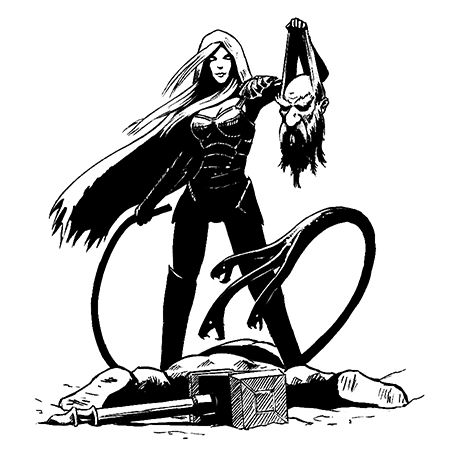
\includegraphics[width=0.7\textwidth,keepaspectratio]{badassWitch.jpg}\par
\vspace{0.4cm}
{\itshape Now that is a badass witch.}\par
\vspace*{\fill}
\end{center}

\end{document}